%!TEX TS-program = xelatex
%!TEX encoding = UTF-8 Unicode
% !Mode:: "TeX:UTF-8"

\documentclass[a4paper,11pt, svgnames, oneside]{scrbook} %如果不加oneside,则奇偶页的边距会不同,以方便装订
\usepackage[a4paper, top=2cm, bottom=2cm, left=2cm, right=2cm]{geometry}
\usepackage{ulem}

\usepackage{xeCJK, fontspec, xunicode, xltxtra, fancybox, setspace,xcolor}
%\usepackage{ fontspec, xunicode, xltxtra, fancybox, setspace,xcolor}

\usepackage{amsmath, amsthm, amsfonts, amssymb, mathrsfs} %数学公式相关 amssymb用于斜体字符,如varnothing,  masthm用于定理, mathrsfs用于花体字母
\newtheorem{theorem}{\hskip 2em \cjkem 定理}[chapter]
\newtheorem{lemma}{\hskip 2em \cjkem 引理}[chapter]
\newtheorem{example}{\hskip 2em \cjkem 例} [chapter]
\renewcommand{\proofname}{\hskip 2em \cjkem 证明}
\usepackage[sort]{natbib}

\usepackage{caption, algorithm} %排版伪代码算法使用
\usepackage[]{algpseudocode}

\floatname{algorithm}{\cjkem{算法}}
\renewcommand{\algorithmicrequire}{\cjkem{输入:}} 
\renewcommand{\algorithmicensure}{\cjkem{输出:}}
\numberwithin{algorithm}{chapter}

\usepackage{colortbl, booktabs, multirow, makecell, longtable} %表格处理相关的Package

\usepackage{tikz, flowchart} % tikz绘图
\usepackage{pgfplots}
\usetikzlibrary{decorations.pathreplacing}
\usetikzlibrary{decorations.markings}
\usetikzlibrary{calc, arrows, arrows.meta, shapes, shadows,  shapes.geometric, positioning}
\usetikzlibrary{topaths}
\usetikzlibrary{mindmap}
\usetikzlibrary{matrix}

\usepackage[tikz]{bclogo}  %see http://mirrors.ctan.org/graphics/bclogo/README
\DeclareGraphicsRule{.mps}{eps}{*}{} %解决xelatex处理bclogo时的mps问题
\newcommand{\infobox}[2]{ 
    \begin{bclogo}[couleur=yellow!10, logo=\bcfleur, ombre=true]{#1}
    #2
    \end{bclogo}
}
\newcommand{\warnbox}[2]{ 
    \begin{bclogo}[couleur=yellow!10, logo=\bctakecare, ombre=true]{#1}
    #2
    \end{bclogo}
}

\newcommand{\shellbox}[1]{ 
    \begin{bclogo}[couleur=gray!10, logo=\bccrayon, ombre=true]{命令}
    #1
    \end{bclogo}
}

%\usetikzlibrary{external} %cache tikz figure, run "xelatex -shell-escape smm.tex" to generate figures
%\tikzset{
%    external/system call={%
%    xelatex \tikzexternalcheckshellescape
%    -halt-on-error -interaction=batchmode --shell-escape
%    -jobname "\image" "\texsource"}}
%\tikzexternalize[prefix=generated/]
%\tikzexternalize[shell escape=-enable-write18]


%\setmainfont[Mapping=tex-text,LetterSpace=-1.25]{Neo Euler}
%\setsansfont[Mapping=tex-text,LetterSpace=-1.25]{}
%\setmonofont[Color=00663300]{Monaco}
\setCJKmainfont{FZLanTingHeiS-EL-GB} %方正字体,也可以改成:微软雅黑
\setCJKsansfont{FZLanTingHeiS-EL-GB} 
\setCJKmonofont{Ubuntu}

\usepackage{listings}
\lstset{breakatwhitespace,
columns=fullflexible,
keepspaces=false,
breaklines,
keywordstyle=\color{blue},
extendedchars=true}


\lstset{breakatwhitespace,
backgroundcolor=\color{white},
columns=fullflexible,
breaklines,
showtabs=true,
tabsize=4,
keepspaces=true,
keywordstyle=\color{blue},
extendedchars=true}


% Definition of JavaScript
\definecolor{lightgray}{rgb}{.9,.9,.9}
\definecolor{darkgray}{rgb}{.4,.4,.4}
\definecolor{purple}{rgb}{0.65, 0.12, 0.82}

\lstdefinelanguage{JavaScript}{
  keywords={typeof, new, true, false, catch, function, return, null, catch, switch, var, if, in, while, do, else, case, break},
  keywordstyle=\color{blue}\bfseries,
  ndkeywords={class, export, boolean, throw, implements, import, this},
  ndkeywordstyle=\color{darkgray}\bfseries,
  identifierstyle=\color{black},
  sensitive=false,
  comment=[l]{//},
  morecomment=[s]{/*}{*/},
  commentstyle=\color{purple}\ttfamily,
  stringstyle=\color{red}\ttfamily,
  morestring=[b]',
  morestring=[b]"
}

\lstset{
   language=JavaScript,
   %backgroundcolor=\color{lightgray},
   extendedchars=true,
   basicstyle=\footnotesize\ttfamily,
   showstringspaces=false,
   showspaces=false,
   numbers=left,
   numberstyle=\footnotesize,
   numbersep=9pt,
   tabsize=2,
   breaklines=true,
   showtabs=false,
   captionpos=t
}


\definecolor{orangered}{RGB}{239,134,64}
\definecolor{tagcolor}{RGB}{0,0,150}
\definecolor{keywordcolor}{RGB}{139,38,201}
\definecolor{attr_value_color}{RGB}{153,51,0}

\lstset{
    language=XML,
    tabsize=4,
    %caption=Code,
    label=code:sample,
    frame=shadowbox,
    rulesepcolor=\color{gray},
    xleftmargin=20pt,
    framexleftmargin=15pt,
    keywordstyle=\color{keywordcolor}\bf,
    commentstyle=\color{gray},
    stringstyle=\color{attr_value_color},    
    tagstyle=\color{tagcolor}\bf,
    markfirstintag=\color{red}\bf,
    numbers=left,
    numberstyle=\tiny,
    numbersep=5pt,
    breaklines=true,
    showstringspaces=false,
    basicstyle=\footnotesize,
    morekeywords={xmlns,version,type,encoding,xml-stylesheet, xs:schema,xs:element,xs:complexType,xs:sequence,xs:attribute}, % list your attributes here
    emphstyle={\color{blue}}}
\renewcommand{\lstlistingname}{Code}



\usepackage{indentfirst}  %首行缩进
\setlength{\parindent}{2em} 
\setlength{\listparindent}{2em} %item列表的段落缩进量

\usepackage{fancyhdr}
\thispagestyle{empty}

% 设置 plain style 的属性
\fancypagestyle{plain}{%
		\fancyhf{} % 清空当前设置

		% 设置页眉 (head)
		\fancyhead[RE]{\leftmark} % 在偶数页的右侧显示章名
		\fancyhead[LO]{\rightmark} % 在奇数页的左侧显示小节名
		\fancyhead[LE,RO]{~\thepage~} % 在偶数页的左侧,奇数页的右侧显示页码

		% 设置页脚:在每页的右下脚以斜体显示书名
		%\fancyfoot[RO,RE]{ {\it Written by Summer XIA}, Email: {\it xiat@ruc.edu.cn}}

		\renewcommand{\headrulewidth}{0.7pt} % 页眉与正文之间的水平线粗细
		\renewcommand{\footrulewidth}{0pt}
}

\pagestyle{fancy} % 选用 fancy style
% 其余同 plain style
\fancyhf{}
\fancyhead[RE]{\leftmark}
\fancyhead[LO]{\rightmark}
\fancyhead[LE,RO]{~\thepage~}
%\fancyfoot[RO,RE]{{\it Written by  Summer XIA}, Email: {\it xiat@ruc.edu.cn}}


%%%%%%%%%% 一些重定义 %%%%%%%%%%
\renewcommand{\contentsname}{目录}     % 将Contents改为目录
\renewcommand{\indexname}{索引}
\renewcommand{\figurename}{图}
\renewcommand{\tablename}{表}
\renewcommand{\appendixname}{附录}

\renewcommand{\bibname}{参考文献}
\let\oldbibliography\thebibliography
\renewcommand\thebibliography[1]{
	\oldbibliography{#1}
	\setlength{\parskip}{0pt}
	\setlength{\itemsep}{0pt plus 0.2ex}
}

\newcommand{\tab}{\phantom{o}\hspace{2ex}}


\usepackage{draftwatermark}
\SetWatermarkText{}%设置水印文字
\SetWatermarkLightness{0.9}%设置水印亮度
\SetWatermarkScale{0.5}%设置水印大小

\usepackage[bookmarks=true]{hyperref} %生成pdf索引
\usepackage{bookmark}

\usepackage{kpfonts}
\usepackage[bf, explicit]{titlesec} %对标题的式样进行设置
\newcommand*\chapterlabel{}
\titlespacing*{\chapter}{0pt}{50pt}{-60pt}
\renewcommand{\chaptername}{}
\titleformat{\section}[hang]{\color{MidnightBlue}\LARGE\bfseries}{\color{MidnightBlue}{\thesection}
}{.8em}{\thesection ~ #1}
\titleformat{\subsection}[hang]{\color{NavyBlue}\Large\bfseries}{\color{NavyBlue}{\thesubsection}
}{.8em}{\thesubsection ~ #1}
\titleformat{\subsubsection}[hang]{\large\bfseries}{\thesubsubsection}{.8em}{\hspace{1em}
  $\blacksquare$ \cjkem \thesubsubsection ~ #1}


%自定义的一些命令,方便使用
\newcommand*\circled[1]{\tikz[baseline=(char.base)]{
  \node[shape=circle,draw,inner sep=1.5pt] (char) {#1};}}


%\newcommand*{\hei}{\fontfamily{FZLanTingHeiS-H-GB}\selectfont}
%\DeclareTextFontCommand{\texthei}{\hei}

\setCJKfamilyfont{FZHei}{FZLanTingHeiS-R-GB}  
\newcommand{\cjkbold}{\color[rgb]{0.29, 0.0, 0.51} \CJKfamily{FZHei}}  %http://latexcolor.com/

\setCJKfamilyfont{FZHeiR}{FZLanTingHeiS-R-GB}  
\newcommand{\cjkem}{\CJKfamily{FZHeiR}} 

\begin{document}

    \frontmatter

    
\titleformat{\chapter}
  {\gdef\chapterlabel{}
   \normalfont\sffamily\Huge\bfseries\scshape}
  {\gdef\chapterlabel{\thechapter\ }}{0pt}
  {
	\begin{tikzpicture}[remember picture,overlay]
	\node[yshift=-4cm] at (current page.north west)
	  {\begin{tikzpicture}[remember picture, overlay]
		\draw[fill=LightSkyBlue!20, draw=black, dashed] (0,0) rectangle
		  (\paperwidth,4cm);
		\node[anchor=east,xshift=.9\paperwidth,rectangle,
			  rounded corners=20pt,inner sep=11pt,draw,
			  fill=white, minimum width=6cm](name)
			  {  {\chapterlabel} \color{black}  #1   };
	   \end{tikzpicture}
	  };
   \end{tikzpicture}
   \vspace{2em}
  }




\usetikzlibrary{calc}
\title{
    \huge{\textcolor{blue}{Python股票分析}} \\ ~ \\
	\begin{tikzpicture}[scale=0.7, transform shape,line width=0.2pt]
	  \foreach \x in {1,...,16}{%
		\pgfmathparse{(\x-1)*45+floor(\x/9)*22.5}
		\node[circle,inner sep=0.25cm,shading=ball, ball color=red!85] (N-\x) at (\pgfmathresult:5.4cm) [thick] {};
	  } 
	  \foreach \x [count=\xi from 1] in {2,...,16}{%
		\foreach \y in {\x,...,16}{%
		    \path (N-\xi) edge[-,draw=red!80, dashed, thick] (N-\y);
	  }
	}
	\end{tikzpicture}
}
\author{
	~\\
	~
}

% General definitions for all Chapters
%-------------------------------------------------------------------------------
% Define Page style for all chapters


% Set double spacing for the text
\doublespacing
%-------------------------------------------------------------------------------


% 1st page for the Title
%-------------------------------------------------------------------------------
\maketitle

%-------------------------------------------------------------------------------
%用于生成罗马计数的前言
\frontmatter


       % include title page
    \chapter*{序言}

xxxx

       % include preface
    %generate book content list
\setcounter{tocdepth}{6}
\tableofcontents
       % include content

    %\include{other}         % include other frontmatter
  

    \mainmatter


			\titleformat{\chapter}
			  {\gdef\chapterlabel{}
			   \normalfont\sffamily\Huge\bfseries\scshape}
			  {\gdef\chapterlabel{\thechapter\ }}{0pt}
			  {
				\begin{tikzpicture}[remember picture,overlay]
				\node[yshift=-5cm] at (current page.north west)
				  {\begin{tikzpicture}[remember picture, overlay]
					\draw[fill=orange!20, draw=black, dotted] (0,0) rectangle
					  (\paperwidth,5cm);
					\node[scale=1.3, rounded corners=5pt, line width=2pt, dotted, draw=orange!80, minimum width=2cm, minimum height=2cm] at (3.5,2.5) {  \color{orange}~$\chapterlabel$ $\hookleftarrow$  };
					\node[anchor=east,xshift=.9\paperwidth,rectangle,
						  rounded corners=20pt,inner sep=11pt,draw,
						  fill=white, minimum width=7cm](name)
						  {  \color{black}  #1   };
				   \end{tikzpicture}
				  };
			   \end{tikzpicture}
				\vspace{4em}
			  }

     
%     \include{chapter/introduction}
     %\part{基础知识}
     \chapter{理论基础}


通过技术指标分析到底能不能预测股票的最大可能走势?这是一个仁者见仁、智者见智的问
题,技术分析派当然对该问题持有确定的回答,并总结了三大基本假设:

\begin{enumerate}
    \item 市场行为包容消化一切消息
    \item 市场运行以趋势方式演变
    \item 历史会重演\footnote{历史总会重演,但历史也并不是简单重复。}
\end{enumerate}


江恩说,大多数人在股市中输钱主要有三个原因:

\begin{itemize}
  \item 交易过度或买卖过于频繁;
  \item 没有上止损单(StoplossOrder);
  \item 对市场知之甚少。
\end{itemize}

     \chapter{技术指标}


\section{MACD}

% Ref: http://stockcharts.com/school/doku.php?id=chart_school:technical_indicators:moving_average_convergence_divergence_macd

以下内容来源于知乎\footnote{
作者:刘鹏程Sai.L \\
链接:https://www.zhihu.com/question/24114669/answer/26849139 \\
来源:知乎 \\
}。

顶背离就是区域A和区域B平均价格相差不大,甚至区域B的最高价高于区域A的最高价,但是
在与之相对应的MACD指标中a点与b点先后出现两个死叉,这两个死叉的相对位置和标的物价
位的相差成明显相反的效果。这一趋势性指标出现后,后市大跌的概率非常高。

{\color{red} MACD的顶背离在我国A股市场中是一个准确率极其高的趋势性指标。}



假设我是一个手握2亿资产的超级投资者,我看好一只总市值在4亿左右的股票,这一只股票
现在的价位是10元每股,我认为这个价格有拉升的空间,那么我就一直在用10元每股的价格,
一点点收集筹码。(当然,实际当中是不可能完全做到的,这里假设的是一个理想状态。)
当我完成了将2亿资金全部换成股票之后,我开始使用种种手段拉升这支股票的价格(具体
手段这里就不详细说了)。最后成功将价格拉升到了20元每股。那么现在我挣钱了么?答案
当然是没有,不仅没有挣钱,我还花掉了我所有的钱,看似2亿的盈利现在都只是一个账面
上的收益,想要真真正正拿到这2个亿的盈利,我必须把我手里的股票全部以20元每股的价
格卖掉。而且我不能一下子卖完,那样的话巨大的卖盘涌现,会使得股票价格快速下滑。我
需要很耐心的使用种种手段将价位稳定在20元每股左右,同时吸引其他人用真金白银将我手
里的股票买过去,把我手上的股票全部转化为现金,那么在盘面上就会看见一个价格高位震
荡一个比较长时间段的情况。当我将全部的股票转化为现金之后,这支股票的持有集中度就
显著下降,没有人刻意维持它的价格,不再有利好消息出现,当一些高位买入希望它进一步
上涨而获利的参与者开始失去耐心,想要卖掉这支股票开始调仓换股的时候,由于没有人托
价,股票价格将开始下跌。一旦下跌幅度加大,或者有利空消息出现,之前的跟风盘将踩踏
式出逃,价格将出现断崖式下跌。同时A股是个被操控性很强的市场,而且大多数股票被拉
升时都大幅超过本身应有价值,没有托盘的情况下,下跌都极为快速。所以MACD的顶背离在
A股市场上极其准确。如果在A股市场上你看见了一支股票在日线或者周线级别出现顶背离的
时候,那么请你立刻想象你自己就是阿甘,这个技术指标就是那个叫珍妮的小女孩,就是阿
甘的妈妈,阿甘在橄榄球场上的队友,阿甘在越战战场上的战友兄弟,他们都在朝你喊着同
一句话 Run,Forrest ! Run away !Hurry! 跑,快跑!不论你买入价位是多少,目前有
没有盈利。先跑出去再看,不要有任何心存侥幸和留恋。

-------------------------------------------

在A股市场中,底背离的正确率远远低于顶背离。再重复一遍,在A股市场中,底背离的正确
率远远低于顶背离。其原因在于,一支股票的价格能在高位长期徘徊而不下跌绝大多数都是
主力在维持这个价格,给出货争取时间这一种情况。而一支股票价格长期爬在地上不动就分
为俩种情况,一,有主力在刻意压制价格长期停留在一个较低的位置,方便于主力以低价收
集筹码。二,这支股票当中的主力全部,彻底的离开了,股价是被由于自身原因涨不上去,
也没有什么可跌的空间了,导致股价长期维持在一个价位。如果是情况二,那么你进入之后
可能很长一段时间都不会有什么像样的涨幅。那么怎么样才能增加顶背离这一信号的预测准
确率腻。

一,观察成交量。有主力介入进行低吸,并且后市将要进行拉升的股票,在低价区徘徊的时
期,成交量一定是温和放大的,因为无论怎样去抑制价格和演示自己进入的痕迹,为了获利,
买入行为时必然存在的,那么成交量上就会相交前期有所变化。

二,依靠时间跨度和指标的重复来增加判断正确率。在A股市场中俩个死叉形成的顶背离一
定要相信,俩个金叉形成的底背离一定要先观察,缓操作。底背离的组成里金叉越多,时间
跨度越大,可信度越高。


关于MACD就先讲到这里,这里特意要说一下,我用的MACD指标一般情况下都不是默认的
(12,26,9)而是改成了(10,20,5)。这么做的目的在于数值改小之后,指标效果会比默认数
值显示的效果超前一点点,同时,由于我选的三个参数都是5的倍数,显示出来的线条不像
默认数值那么圆润,而是比较锐利一点,这样交叉等重要情况在图形中看起来更加显眼。


\section{MA均线系统和BOLL布林带}
在我们通过趋势性指标寻找到一些上升趋势良好的股票之后,我们可以观察,也可以尝试去
买入一些,之后如果我们的判断没有大的漏洞的话。我们将看到这支股票的价格沿趋势开始
上涨。但是现在新的问题出现了,没有什么东西的价格会一直不停的涨下去,那么价格的波
动出现的时候,是短期的一个调整还是上涨结束了腻?有了盈利的股票需要什么时候思考出
售的问题?这里就需要借助一些压力与支撑类的指标。我个人寻找压力与支撑往往用均线和
布林俩个指标。当然在教科书上,他们俩个不是被定义为压力与支撑指标的。所以这里我讲
讲我的用法。

MA均线可能是所有指标中出现最早的一个指标了,只要一打开交易软件,它都会伴随着K线
图出现在我们眼前。它的原理简单到不能再简单,关于均线的运用也有无数的提法。可能是
太习以为常,我认识的很多人往往都关注那些一听起来就不明觉厉的指标,常常忽视了均线。


作者:水湄物语
链接:https://www.zhihu.com/question/24114669/answer/104567719
来源:知乎
著作权归作者所有。商业转载请联系作者获得授权,非商业转载请注明出处。

一位朋友被一段恋情折磨多年,那女人一次次欺骗他。虽然再跟这个女人维持关系,已经没有意义了,他还是一次次接受了她。
我问起他时,他说,他在这段感情里投入了这么多,现在却要放弃,是错误的。

电影很无聊,一个小时候,我跟朋友说,“走吧,我们回去吧。”她回答:“不行,不能白花这100块钱买电影票。”

以上是两个常见的纠缠沉没成本的例子。
继续纠结于沉没成本,只会让你付出更多的代价:再被那女人伤害几次,再浪费1小时在无聊电影上。同时,错过了寻找下一个好女人的机会。

股票投资者,经常成为沉没成本的受害者。
当他们看好的某只股票亏损之后,即便知道这只股票前景不妙,仍然抱住不放,不舍得斩仓出局。

这是不明智的,你过去赚了/亏了多少,一点都不重要。重要的是,股票未来的前景和走势。
要想摆脱这种谬误,需要理解为什么我们会纠结于沉没成本。

3) 短期记忆:
表现为我们更注重短期的记忆,而不是遥远的以前发生的事情。

人类的记忆力是非线性的,这已经被科学证实。
中国股市6000点的时候,有几个人还记得历次股灾——尽管随便打开一个资料,都能看到,历史上暴跌过N次。
但是……上个月大盘涨了15%噢!我的股票上周涨停了2次!……这些短期记忆,不断在洗刷我们的长期记忆。于是我们信心满满,认为眼前所见的一切将永久持续下去。

帕斯卡说过,人类的头脑既是宇宙的光荣,也是宇宙的耻辱。
其他误判包括:幸存者偏差、膀胱效应、心理锚定、风险厌恶、权威偏误……等等。

推荐书目:《清醒思考的艺术》。
这是一本很有趣的读物,可以避免你的思维被污染。


\section{布林线}

布林线是由美国交易者约翰布林格所创并且推广. 其主要的原理就是基本的概率分布: 先假
设价格会围绕一个均值上下波动, 然后利用统计标准差, 再根据概率分布理论来计算价格波
动的范围, 这个均值就是布林线的中轨, 而波动的范围就是布林线的上轨与下轨.

算法与参数设置

布林线的算法很简单, 我们先取一条中轨做基础, 原版的布林线选取的是20日简单移动平均
线, 然后我们再设定一个N倍标准差来做波动范围参数, 原版布林线设定的是2倍标准差, 最
后, 我们用中轨分别加减N倍标准差得出上轨与下轨, 从图表上看, 就是一个通道指标!

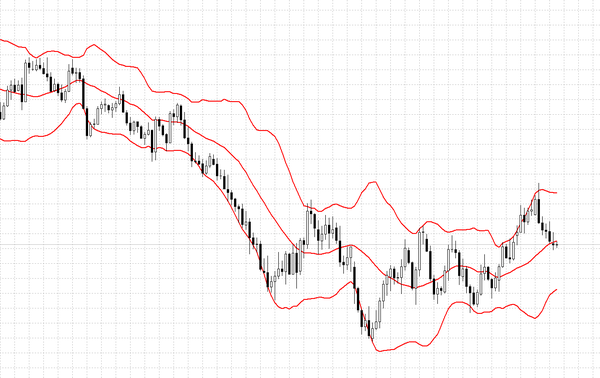
\includegraphics[width=\textwidth]{figure/boll1.png}

由于布林线有两个设置参数, 这样就决定了布林线有无数种变化! 我们既可以设置一条不同
参数的中轨(甚至还可以去编译一条中轨), 又可以选择不同倍数的标准差来做出上下轨!

不同的参数设置有着不同的应用方法, 这里只介绍一些最基本的用法!
1) 判断压力与支撑
当我们设置好布林线通道时, 第一个感觉就是价格大部分时间都在通道中波动, 这样, 我们
很自然地就认为布林线的上轨就是压力区, 布林线的下轨就是支撑区, 这是一种最常见的用
法. 如图

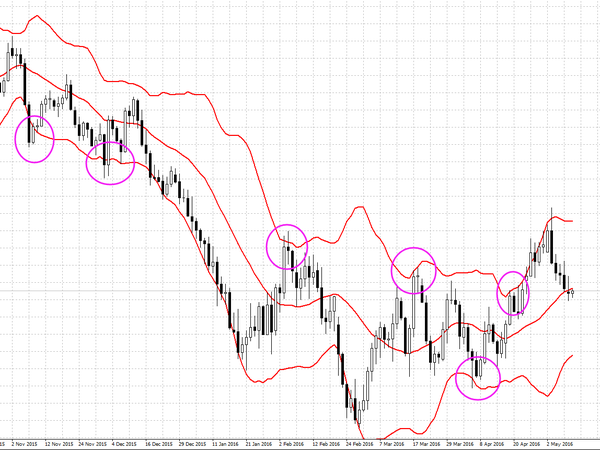
\includegraphics[width=\textwidth]{figure/boll2.png}

2) 识别趋势
布林线还有一个主要的用法是识别趋势. 使用布林线的交易者一般都会以中轨作为多空分界,
其实, 布林线还有一个特别重要的用法----行走在布林线上! 当价格波动到上下轨甚至超过
上下轨时, 价格很容易出现单边上涨或下跌的走势, 从布林线的形态上来看, 就是价格始终
都压在上轨或下轨上! 如图

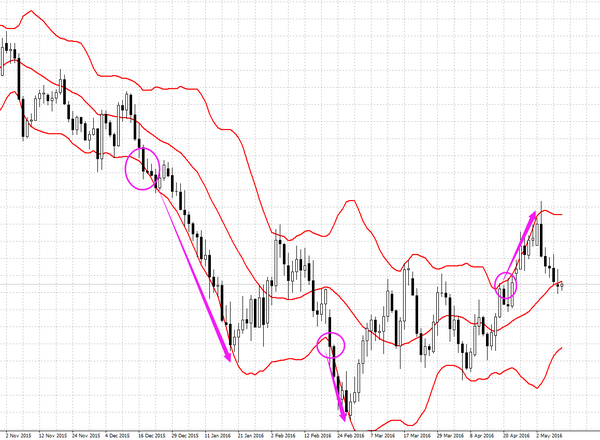
\includegraphics[width=\textwidth]{figure/boll3.png}



    \appendix
    %\include{history}       % include first appendix
    %\include{tables}        % include second appendix, etc.
    
    
	\backmatter

		\titleformat{\chapter}
		  {\gdef\chapterlabel{}
		   \normalfont\sffamily\Huge\bfseries\scshape}
		  {\gdef\chapterlabel{\thechapter\ }}{0pt}
		  {
			\begin{tikzpicture}[remember picture,overlay]
			\node[yshift=-4cm] at (current page.north west)
			  {\begin{tikzpicture}[remember picture, overlay]
				\draw[fill=LightSkyBlue!20, draw=black, dashed] (0,0) rectangle
				  (\paperwidth,4cm);
				\node[anchor=east,xshift=.9\paperwidth,rectangle,
					  rounded corners=20pt,inner sep=11pt,draw,
					  fill=white, minimum width=6cm](name)
					  {  {\chapterlabel} \color{black}  #1   };
			   \end{tikzpicture}
			  };
		   \end{tikzpicture}
			\vspace{2em}
		  }
	
	\bibliographystyle{plain}
	\bibliography{bibliography}
    %\begin{thebibliography}{999}
\bibitem {bib:Chris2005} Chris Burges, Tal Shaked, Erin Renshaw, Ari Lazier, Matt Deeds, Nicole Hamilton, and Greg Hullender. 2005. Learning to rank using gradient descent. Proceedings of the 22nd international conference on Machine learning (ICML '05). ACM, New York, NY, USA, 89-96. 

\end{thebibliography}
  % include bibliography
    %\include{index}         % include index
    \chapter*{致谢}

Life has taugh us that love does not consist in gazing at each other but in
looking outward together in the same direction.





\end{document}

%%% Local Variables:
%%% mode: latex
%%% TeX-master: t
%%% End:
